\begin{activity}{Nevada Gravity: Filtering for Sediments}

\section*{Purpose}

This activity applies the ideas from your pre-workshop viewing and from the Fold Belt Survey to real, messy, spatial potential-field data. The focus is on understanding how sampling, filtering, and physical assumptions control what geological information can actually be recovered from gravity data -- not in a synthetic model where you know the answer, but in a real dataset where you don't.

The activity progresses deliberately:
\begin{itemize}
  \item real Complete Bouguer gravity data from Nevada (2~km grid spacing, Basin-and-Range Province),
  \item to spectral interpretation of the basin-scale signal,
  \item to spectral high-pass filtering,
  \item and finally to inversion for sediment thickness.
\end{itemize}

\section*{Learning Outcomes}

By the end of this activity, you should be able to:
\begin{itemize}
  \item Distinguish a genuine basin-scale spectral signal from the red-noise background expected in any potential field, by comparing a spectrum against a background power-law fit rather than against zero.
  \item Justify the pass/block wavelengths of a high-pass filter using evidence from the data's own spectrum, and explain what geological assumption that choice encodes.
  \item Critically evaluate an inverted geophysical product (sediment thickness) by tracing it back to the sampling, filtering, and density assumptions that produced it, and sanity-check it against independent geological knowledge.
\end{itemize}

\section*{Tasks}

At each stage, ask yourself the same question you asked in the Fold Belt Survey: \emph{does this result actually reflect the geology, or could it be an artefact of how the data were sampled and processed?}

\begin{questions}
    \question{Nevada Complete Bouguer Gravity}
        The Complete Bouguer anomaly corrects for the free-air effect of elevation, the gravitational attraction of the rock slab beneath each station, and nearby terrain. What remains reflects lateral density variations in the crust and upper mantle.

        \begin{figure}[h]
            \centering
            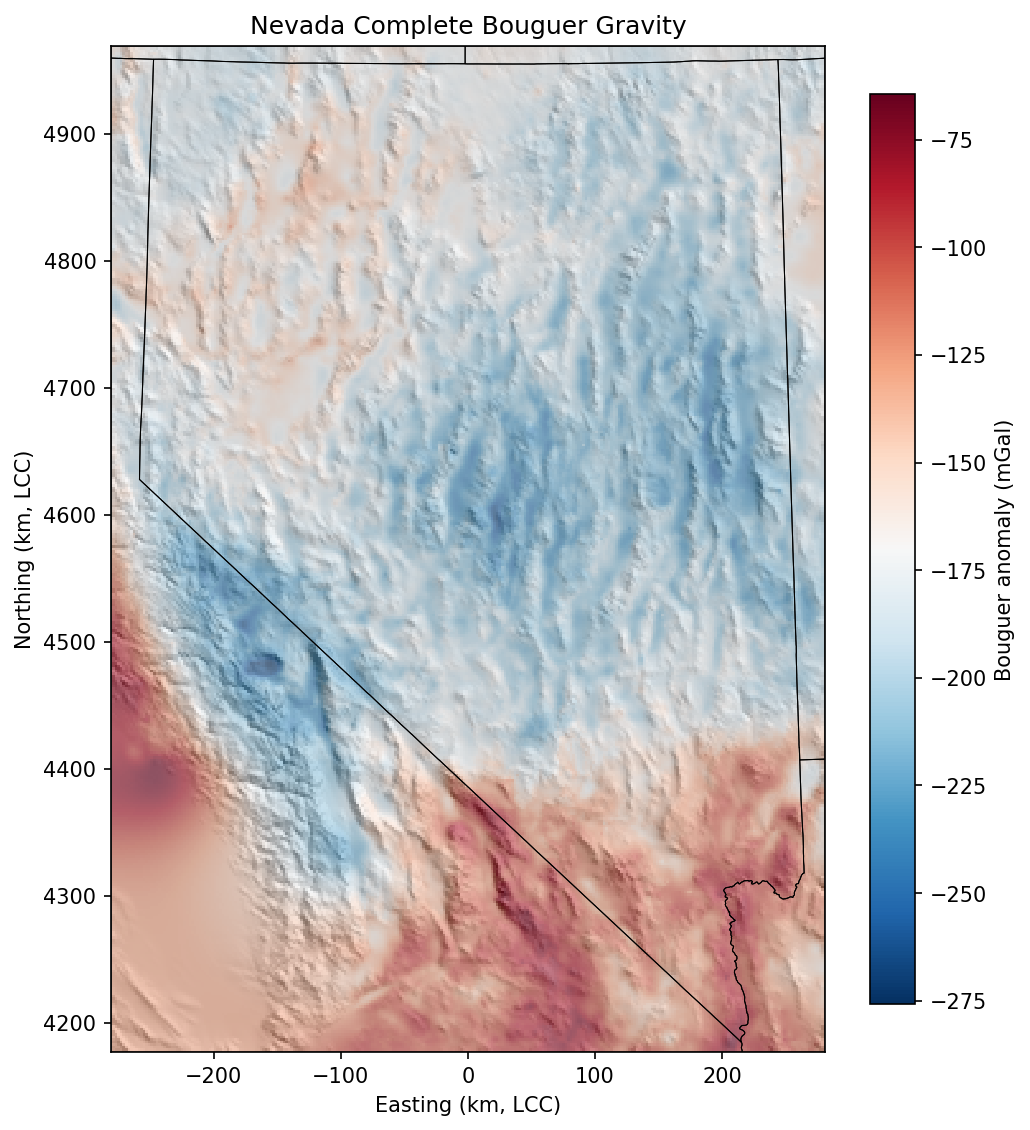
\includegraphics[width=0.7\textwidth]{figures/01_nevada_bouguer_map.pdf}
            \caption{Bouguer gravity anomaly map of Nevada, USA.}
            \label{fig:fft_bg_map}
        \end{figure}

        \begin{enumerate}[label=\roman*]
            \item Describe the large-scale pattern in one or two sentences. Is there a dominant trend, and if so, which direction does it run?
            \answerbox[2cm]

            \item Look for the shorter-wavelength ``stripes'' superimposed on that trend. Roughly how would you describe their scale compared to the overall map -- tens of kilometres, or hundreds?
            \answerbox[2cm]

            \item Based on the Fold Belt Survey, what would you need to know about this map's station spacing before trusting any wavelength you read off it by eye?
            \answerbox[2cm]
        \end{enumerate}

    \question{Spatial Fourier Transform \& Spectral Analysis}
        For a uniformly sampled profile, the discrete Fourier transform gives
        \[
            \hat{g}(k_n) = \sum_{j=0}^{N-1} g(x_j)\, e^{-i 2\pi k_n x_j},
            \qquad k_n = \frac{n}{N\,\Delta x}.
        \]

        The amplitude spectrum $|\hat{g}(k)|$ shows how much power exists at each wavelength. For potential fields, spectra typically show a \emph{red-noise} background: power increases systematically toward longer wavelengths, simply because deeper and larger sources dominate the long-wavelength end -- the same wavelength--depth relationship from this morning's warm-up.

        \begin{figure}[h]
            \centering
            
\includegraphics[width=0.85\textwidth]{figures/03_bouguer_profile_raw.pdf}
            \caption{Raw E--W Bouguer gravity profiles across Nevada.}
            \label{fig:fft_bg_profile}
        \end{figure}

        \begin{figure}[h]
            \centering
            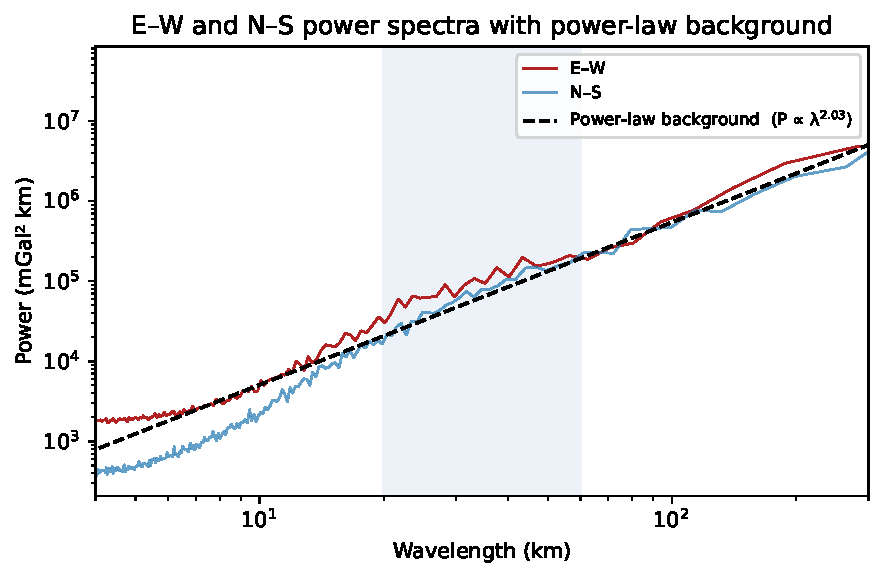
\includegraphics[width=0.85\textwidth]{figures/04_power_spectra_ew_ns.pdf}
            \caption{Power spectrum in the E--W (red) and N--S (blue) directions.  The black dashed line is a fit to the long period power, used to identify high-frequency surface topographic wavelengths, likely dominated by basins.}
            \label{fig:fft_power_spectra}
        \end{figure}

        \begin{enumerate}[label=\textbf{\arabic*.}, resume]
            \item The profile shows a large-amplitude, slowly-varying ramp with shorter-wavelength wiggles riding on top. Which part of that profile do you expect the power spectrum to be dominated by, and does the spectrum confirm it?
            \answerbox[2cm]

            \item The E--W and N--S spectra don't overlie each other. What does that difference tell you about basin geometry, independent of any map?
            \answerbox[2cm]
        \end{enumerate}

    \question{Separating Signal from Background}
        Because potential-field spectra are red-noise by default, a raw spectral peak is not automatically meaningful -- it needs to be compared against the background trend expected even in the absence of any discrete basin-scale source. A power law is fit to wavelength ranges well outside the basin band (6.2--10~km and 80--120~km) to describe that background.

        \begin{figure}[h]
            \centering
            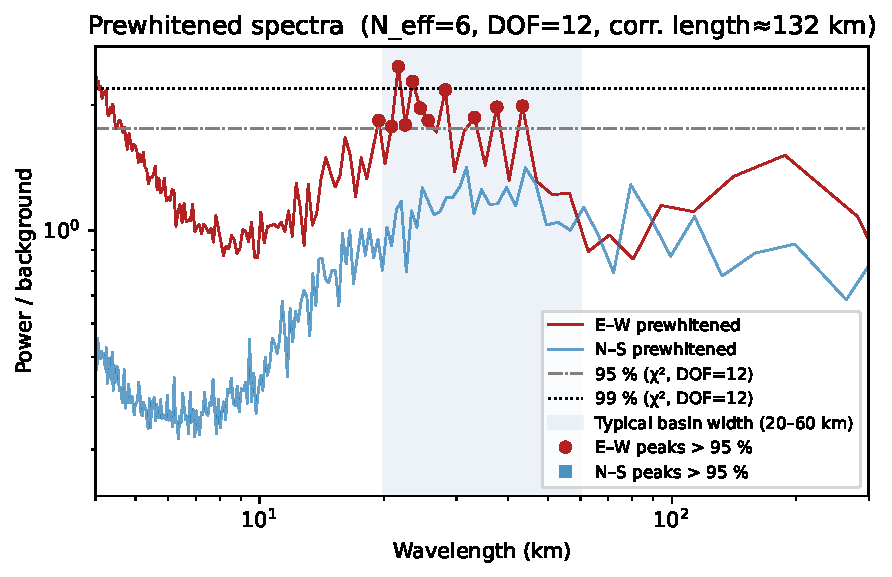
\includegraphics[width=0.85\textwidth]{figures/05_power_spectra_background.pdf}
            \caption{Identification of resolvable spectral peaks.}
            \label{fig:fft_bg}
        \end{figure}

        \begin{enumerate}[label=\roman*]
            \item Why anchor the power-law fit \emph{outside} the 20--60~km band rather than fitting it to the whole spectrum? What would go wrong if the fit were allowed to use the basin-band wavelengths too?
            \answerbox[2.5cm]

            \item Where does the E--W spectrum depart most clearly from the background, and does that match the basin width you estimated from the map in Question 1?
            \answerbox[2cm]
        \end{enumerate}

% ----------------------------------------------------------------------
% NOTE (commented out, not deleted): an Airy isostatic correction was
% originally planned here as a physically motivated way to remove the
% long-wavelength regional signal before spectral/filtering analysis.
% It was dropped because it doesn't do anything the high-pass filter
% below doesn't already do -- and using it would still have required an
% additional high-pass filter afterward to remove what the isostatic
% correction leaves behind, so it added a step without removing one.
% Kept here in case a future redesign wants to reinstate a physically
% motivated (rather than purely spectral) regional-removal step.
% ----------------------------------------------------------------------
% \iffalse
% \section*{Airy Isostatic Gravity Correction}

% The long-wavelength Bouguer gravity field over Nevada is dominated by
% isostatic compensation of crustal thickness variations.
% Under Airy isostasy, surface loads are compensated by a crustal root at depth $T_0$.

% In the spectral domain, the gravity effect of a density interface at depth $T_0$ is
% \[
%     \hat{g}_{\text{root}}(\mathbf{k})
%     =
%     2\pi G\, \Delta\rho \, \hat{h}(\mathbf{k}) \, e^{-|\mathbf{k}| T_0},
% \]
% where $\Delta\rho$ is the density contrast across the Moho and $e^{-|\mathbf{k}|T_0}$ is the upward-continuation filter.

% Subtracting this predicted root contribution from the observed Bouguer gravity yields
% the \emph{isostatic residual}:
% \[
%     g_{\text{iso}} = g_{\text{Bouguer}} - g_{\text{root}}.
% \]
% \fi

    \question{High-Pass Filtering}
        Before inverting gravity for sediment thickness, the long-wavelength regional trend must be removed -- otherwise broad regional lows get misread as implausibly thick sediment. A smooth raised-cosine (Hann) high-pass filter is used instead of a sharp cutoff, to avoid Gibbs ringing:
        \begin{equation}
        H(k) =
            \begin{cases}
                0, & k \le k_{\text{lo}}, \\
                \dfrac{1}{2}\left[1 - \cos\!\left(\pi \dfrac{k - k_{\text{lo}}}{k_{\text{hi}} - k_{\text{lo}}}\right)\right], & k_{\text{lo}} < k < k_{\text{hi}}, \\
                1, & k \ge k_{\text{hi}}.
            \end{cases}
        \end{equation}
        Wavelengths $> 100$~km are fully blocked, wavelengths $< 60$~km are fully passed, and the intermediate range is smoothly tapered.

        \begin{figure}[h]
            \centering
            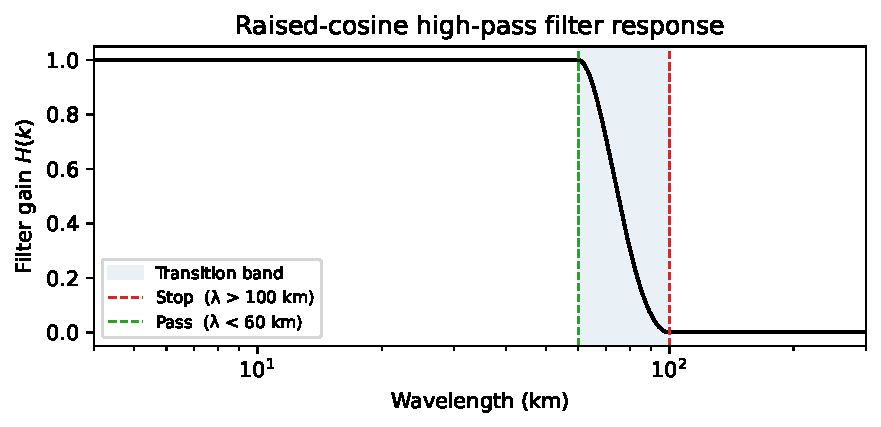
\includegraphics[width=0.7\textwidth]{figures/05b_highpass_filter_curve.pdf}
            \caption{Raised-cosine high-pass filter gain $H(k)$ as a function of wavelength.}
            \label{fig:fft_hp_curve}
        \end{figure}

        \begin{figure}[h]
            \centering
            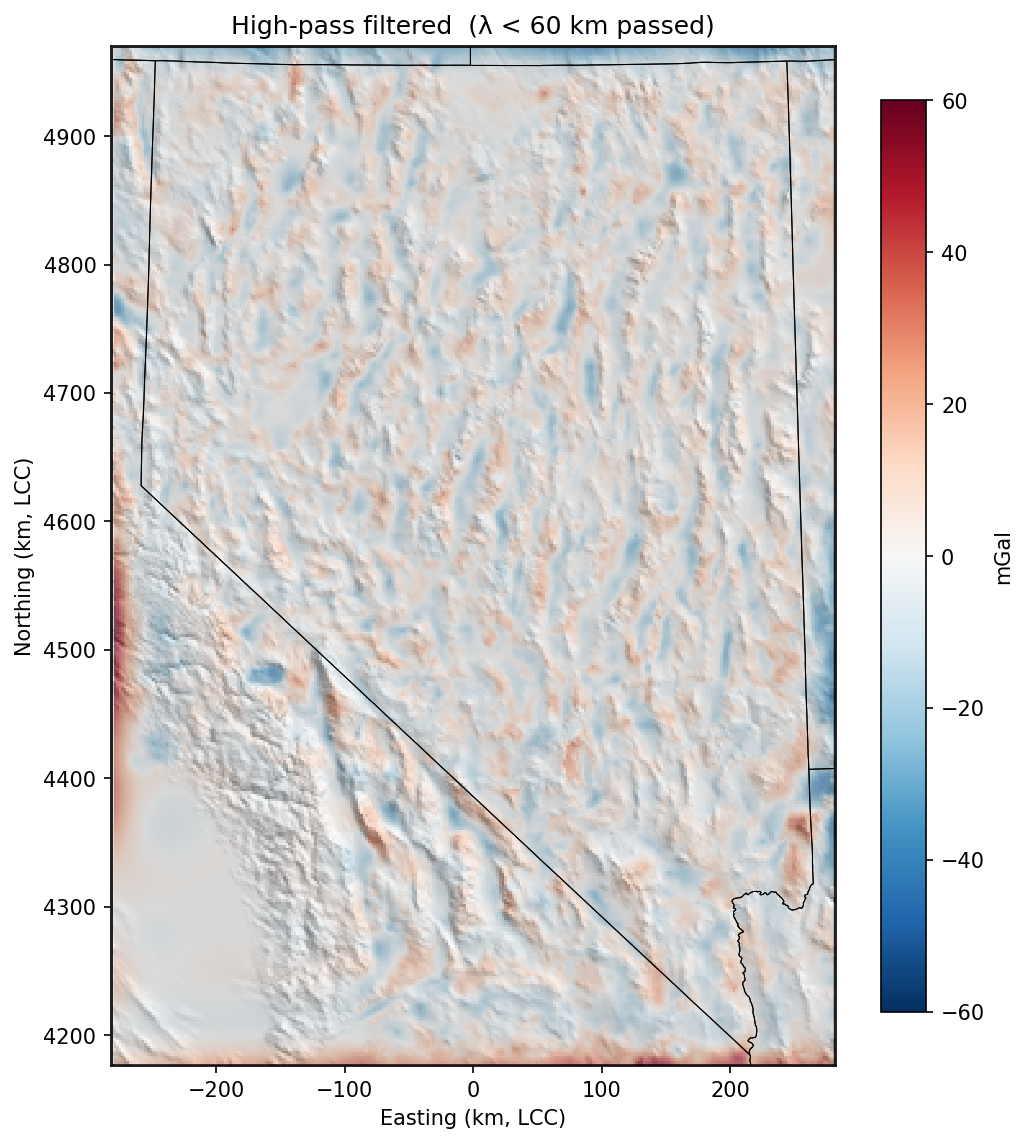
\includegraphics[width=0.7\textwidth]{figures/06_highpass_filtered_map.pdf}
            \caption{High-pass filtered gravity anomaly map of Nevada.}
            \label{fig:fft_hp}
        \end{figure}

        \begin{figure}[h]
            \centering
            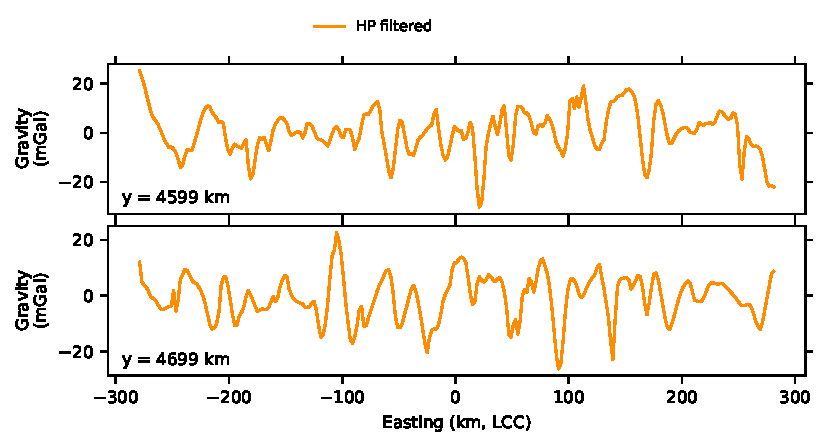
\includegraphics[width=0.85\textwidth]{figures/07_bouguer_vs_hp_profile.pdf}
            \caption{E--W high-pass filtered gravity anomaly.}
            \label{fig:fft_hp_profile}
        \end{figure}

        \begin{enumerate}[label=\roman*]
            \item The filter's pass/block wavelengths (100~km and 60~km) were chosen using information from Figure~\ref{fig:fft_power_spectra}. What did it tell you?
            \answerbox[2.5cm]

            \item In your own words: what geological assumption is encoded by choosing 100~km and 60~km specifically, rather than some other pair of numbers?
            \answerbox[2.5cm]
        \end{enumerate}

    \question{Sediment Thickness Inversion}
        The filtered gravity is now inverted for sediment thickness $h(x,y)$, treating sediment as a single layer of uniform density overlying denser basement: $$\Delta\rho = \rho_{\text{basement}} - \rho_{\text{sediment}} \approx 170~\text{kg m}^{-3}.$$ This is a deliberate simplification -- gravity is most sensitive to the largest density contrast and cannot resolve fine internal stratigraphy, so the result captures the dominant mass deficit of basin fill rather than a detailed stratigraphic column.

        For an interface with mean depth $z_0$ and relief $h(x,y)$, the linearized forward model in the Fourier domain is
        \[
            \hat{g}(\mathbf{k}) = 2\pi G\,\Delta\rho \; e^{-|\mathbf{k}| z_0} \; \hat{h}(\mathbf{k}),
        \]
        where $e^{-|\mathbf{k}| z_0}$ is the upward-continuation kernel -- short wavelengths decay rapidly with depth, so gravity is inherently band-limited by source depth.

        Formally inverting this relation gives
        \[
            \hat{h}(\mathbf{k}) = \frac{\hat{g}(\mathbf{k})}{2\pi G\,\Delta\rho} \; e^{|\mathbf{k}| z_0}.
        \]
        The factor $e^{|\mathbf{k}| z_0}$ \emph{amplifies} high-wavenumber components, so noise, discretization error, and aliasing are all dramatically magnified, a naive downward continuation is unstable and physically meaningless.

        The Parker--Oldenburg method (Parker, 1973; Oldenburg, 1974) addresses this by treating the gravity--interface relationship as weakly nonlinear and solving iteratively in the spectral domain: start with a guess for $h(x,y)$, forward-calculate the predicted gravity, compare to the observed (filtered) gravity, update the interface estimate, and repeat until convergence. Each iteration uses an FFT, at cost $O(N\log N)$.

        \begin{figure}[h]
            \centering
            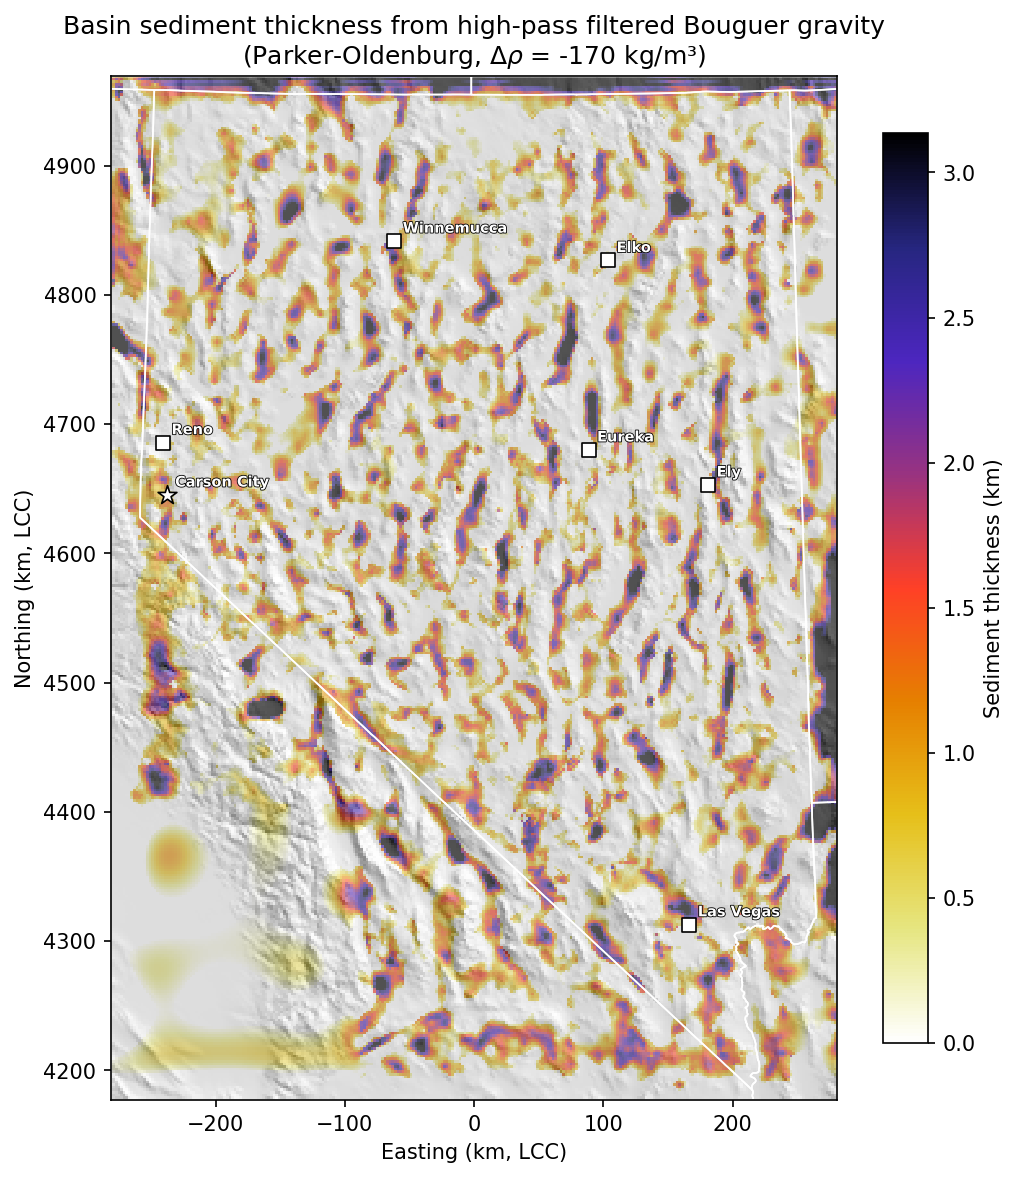
\includegraphics[width=0.7\textwidth]{figures/08_sediment_thickness_map.pdf}
            \caption{Inverted sediment thickness using the Parker--Oldenberg method, assuming a density deficit of \SI{170}{kg.m^{-3}}.}
            \label{fig:fft_sed_thick}
        \end{figure}

        \begin{enumerate}[label=\roman*]
            \item Several Nevada cities are marked on the map. Does the sediment thickness pattern near them match what you'd expect from their locations (valley floor vs.\ mountain range)?
            \answerbox[2.5cm]

            \item The inversion is not unique, and $h(x,y)$ is conditional on the sampling, filtering, and density assumptions made along the way. Name one specific assumption made earlier in this activity that, if wrong, would change this map\ldots and say which direction the thickness estimate would move.
            \answerbox[2.5cm]
        \end{enumerate}

    \question{Checking Against Known Geology}
        \begin{figure}[h]
            \centering
            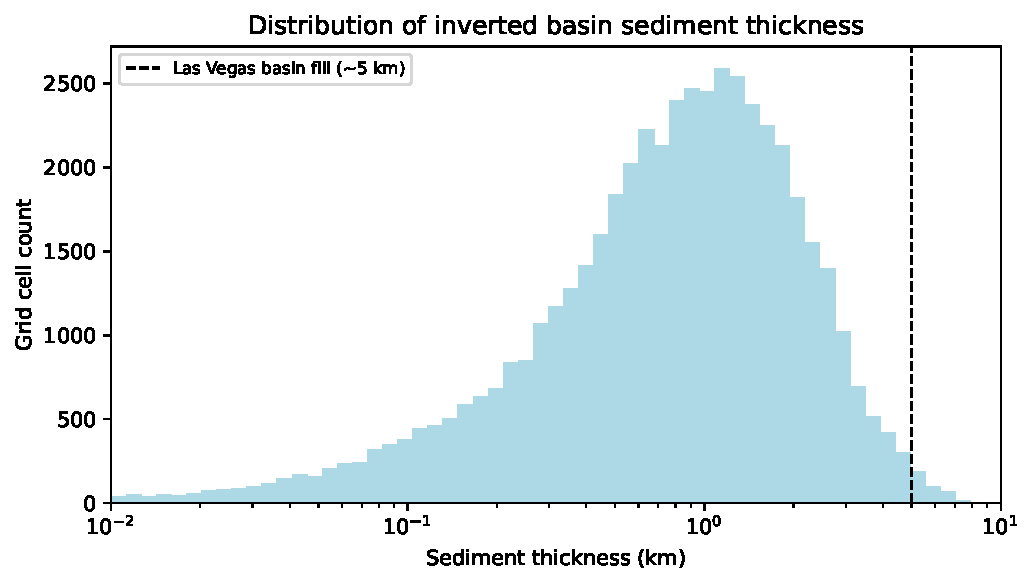
\includegraphics[width=0.75\textwidth]{figures/09_sediment_thickness_distribution.pdf}
            \caption{Histogram of estimated sediment thicknesses.}
            \label{fig:fft_sed_thick_hist}
        \end{figure}

        Las Vegas Valley's basin fill is independently documented (seismic and well data) at roughly 5~km.

        \begin{enumerate}[label=\roman*]
            \item Where does the bulk of the distribution sit relative to that 5~km reference line? Does the inversion look broadly plausible?
            \answerbox[2cm]

            \item A small tail of cells reaches toward 8~km -- deeper than any well-documented Nevada basin. Given what you now know about the high-pass filter's 60--100~km transition band, suggest a physical reason those specific cells might be overestimated rather than genuinely that deep.
            \answerbox[2.5cm]
        \end{enumerate}
\end{questions}

% \section*{8. Impact of Aliasing on the Inversion}

% The station-spacing comparison from Section 2 showed aliasing in the raw data and its spectrum. This section reruns the \emph{entire} pipeline -- high-pass filter, then Parker--Oldenburg inversion -- on decimated data, so you can see how aliasing propagates all the way through to the final geological product.

% \begin{center}
%     \includegraphics[width=\textwidth]{figures/10a_pipeline_aliasing_resolved.pdf}
% \end{center}

% \begin{center}
%     \includegraphics[width=\textwidth]{figures/10b_pipeline_aliasing_aliased.pdf}
% \end{center}

% \begin{enumerate}[label=\textbf{\arabic*.}, resume]
%     \item Compare the two sediment-thickness maps. Is the degradation in the aliased case simply ``blurrier,'' or does it introduce structure that looks like a real geological feature but isn't? Point to a specific example.

%     \answerbox[2.5cm]

%     \item \textbf{The key question:} suppose someone handed you \emph{only} the aliased sediment-thickness map, with no access to the original station data. Is there anything about the map alone that would tip you off that it's unreliable -- or does it look just as plausible as the resolved version?

%     \answerbox[2.5cm]

%     \item No amount of algorithmic sophistication in the inversion step can recover a wavelength that aliasing has already destroyed at the sampling step. Restate, in your own words, why that ordering -- sampling first, everything else second -- matters for how you'd plan a real field survey.

%     \answerbox[2.5cm]
% \end{enumerate}

\section*{Key Ideas}
\begin{itemize}
    \item A spectral peak is only meaningful relative to the red-noise background expected from any potential field; compare against a background fit, not against zero.
    \item Filtering choices (here, the 60--100~km transition band) encode geological assumptions and propagate directly into the final inverted product.
\end{itemize}

\end{activity}
